\let\negmedspace\undefined
\let\negthickspace\undefined
\documentclass[journal]{IEEEtran}
\usepackage[a5paper, margin=10mm, onecolumn]{geometry}
%\usepackage{lmodern} % Ensure lmodern is loaded for pdflatex
\usepackage{tfrupee} % Include tfrupee package

\setlength{\headheight}{1cm} % Set the height of the header box
\setlength{\headsep}{0mm}     % Set the distance between the header box and the top of the text

\usepackage{gvv-book}
\usepackage{gvv}
\usepackage{cite}
\usepackage{amsmath,amssymb,amsfonts,amsthm}
\usepackage{algorithmic}
\usepackage{graphicx}
\usepackage{textcomp}
\usepackage{xcolor}
\usepackage{txfonts}
\usepackage{listings}
\usepackage{enumitem}
\usepackage{mathtools}
\usepackage{gensymb}
\usepackage{comment}
\usepackage[breaklinks=true]{hyperref}
\usepackage{tkz-euclide} 
\usepackage{listings}
% \usepackage{gvv}                                        
\def\inputGnumericTable{}                                 
\usepackage[latin1]{inputenc}                                
\usepackage{color}                                            
\usepackage{array}                                            
\usepackage{longtable}                                       
\usepackage{calc}                                             
\usepackage{multirow}                                         
\usepackage{hhline}                                           
\usepackage{ifthen}                                           
\usepackage{lscape}
\begin{document}

\bibliographystyle{IEEEtran}
\vspace{3cm}

\title{1.6.6}
\author{AI24BTECH11036 - Yadlapally Shreedhanvi}
% \maketitle
% \newpage
% \bigskip
{\let\newpage\relax\maketitle}

\renewcommand{\thefigure}{\theenumi}
\renewcommand{\thetable}{\theenumi}
\setlength{\intextsep}{10pt} % Space between text and floats


\numberwithin{equation}{enumi}
\numberwithin{figure}{enumi}
\renewcommand{\thetable}{\theenumi}


\textbf{Question}:In each of the following, find the value of k, for which the points are collinear.\\
a) (7, -2), (5, 1), (3, k)\\
b) (8, 1), (k, -4), (2, -5)\\ \\

\textbf{Solution: }

\begin{table}[h!]    
  \centering
  \begin{tabular}[12pt]{ |c| c|}
    \hline
    \textbf{Label} & \textbf{Co-ordinate}\\ 
    \hline
	\multicolumn{2}{|c|}{\textbf{Case (a)}}\\
	\hline
    $\vec{A}$ & $\brak{7, -2}$ \\
    \hline 
    $\vec{B}$ & $\brak{5, 1}$ \\
    \hline
    $\vec{C}$ & $\brak{3, k}$ \\
    \hline
	\multicolumn{2}{|c|} {\textbf{Case (b)}}\\
	\hline
    $\vec{A}$ & $\brak{8, 1}$ \\
    \hline 
    $\vec{B}$ & $\brak{k, -4}$ \\
    \hline
    $\vec{C}$ & $\brak{2, -5}$ \\
    \hline 
    \end{tabular}

  \caption{Co-ordinates}
  \label{tab1.6.6.1}
\end{table}

For the points $\vec{A}$, $\vec{B}$  and  $\vec{C}$ to be collinear,
\begin{align}
	\text{rank} \myvec{ \vec{B-A} & \vec{C-A}}=1
\end{align}
In case (a)
\begin{align*}
\myvec{ \vec{B-A} & \vec{C-A}}=\\
\myvec{ -2 & -4 \\ 3 & k+2} 
\xleftrightarrow[]{R_2 \leftarrow {3R_1+2R_2}}
\myvec{-2 & -4 \\ 0 & -8+2k} \\
\text{Since the rank of the above matrix should be 1,}
-8+2k=0\\
\therefore k=4.
\end{align*}
In case (b)
\begin{align*}
\myvec{ \vec{B-A} & \vec{C-A}}=\\
\myvec{ k-8 & -6 \\ -5 & -6} 
\xleftrightarrow[]{R_2 \leftarrow {R_1-R_2}}
\myvec{k-8 & -6 \\ k-3 & 0} \\
\text{Since the rank of the above matrix should be 1,}
k-3=0\\
\therefore k=3.
\end{align*}







\begin{figure}[h!]
   \centering
   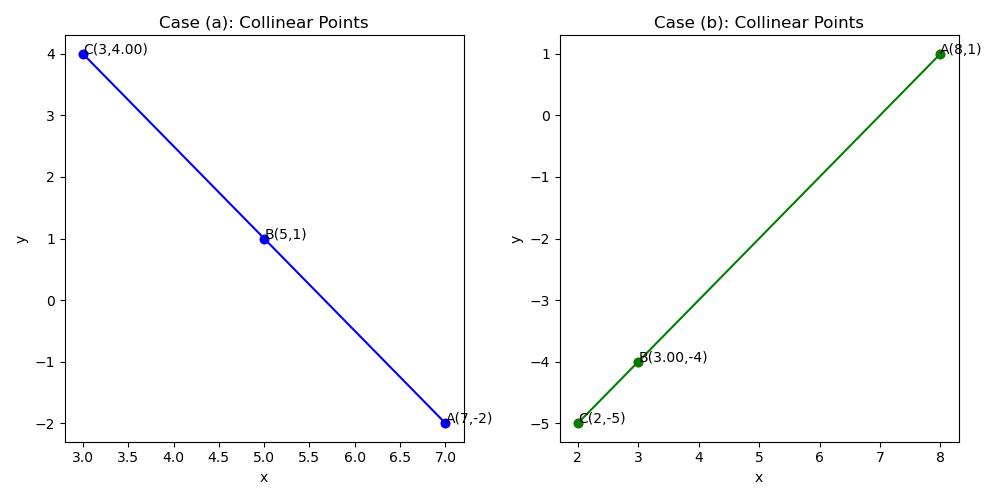
\includegraphics[width=0.7\linewidth]{figs/Figure_1.png}
   \caption{Plots of Lines}
   \label{plot}
\end{figure}
\end{document}  
\end{document}


